\subsection{Experiment 1 Analysis Results} \label{results-1-quan}
In this section, 
we will first present descriptive statistics 
of the raw data in our first experiment. 
Then, we will explain our feature engineering 
and data transformation process 
based on the raw data. 
Lastly, we will introduce the Bayesian Model 
we applied in our analysis 
and present the analysis results.

\subsubsection{Descriptive Statistics of the Raw Data}
% -- raw data
%     describe the dataset, total # of participants in each group before and after dataset cleaning, demographics of each group;
    
Overall, we collected 223 complete responses in the first experiment. We removed 4 responses after checking the quality of the responses due to reasons such as not answering the qualitative question seriously or misunderstanding the prompt. Among the 219 remaining responses, 56 completed the Likert path, and the rest were distributed relatively evenly across the remaining 6 paths with various orders of QV, ranging from 24 to 28 responses per path. Aggregating responses from all 6 paths, the number of responses we got for QV with 36 credits (QV36), QV with 108 credits (QV108) and QV with 324 credits (QV324) were 107, 108, and 111 respectively. (To-do: maybe add a hierarchical graph the represents how responses from different paths are aggregated)

We recruited the participants with the goal of constructing a sample that was representative of the US census data in terms of age and education level. Having a representative sample is in particularly critical in our study because these voting and survey tools should aim to be designed for the general population. Based on Table \ref{fig:demo_exp1}, all the groups closely followed the demographics of the US population in both age and education level. This ensured that our results were not biased to a certain subgroup of the population, which is generally hard to achieve in MTurk studies without specific control. 


\begin{figure}[htpb]
    \centering
    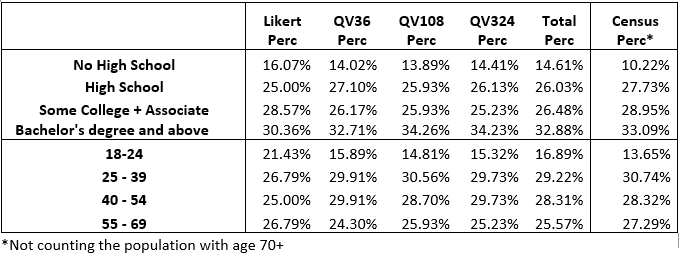
\includegraphics[width=0.7\textwidth, keepaspectratio=true]{content/image/demographics_table.png}
    \caption{
        Sample Demographics Statistics Compared to US Census Data (Will fix into a table later)
    }
    \Description[Sample Demographics Statistics Compared to US Census Data for experiment 1]{Sample Demographics Statistics Compared to US Census Data for experiment 1}
    \label{fig:demo_exp1}
\end{figure}
    
%     donation descriptive statistics: perc of non-zero donation, total donation amount comparison across groups, donation distribution across topics between groups

In this experiment, each set of survey responses by a participant in a condition could be matched to the set of donation decisions made by the same participant. Since we would like to use the donation outcome of a participant as a proxy of his/her true preferences across the nine charity topics, we could only do so with participants that donated a non-zero amount of money. Therefore, we further filtered the dataset to keep only the responses that had a non-zero total donation amount. Across all the conditions, the average non-zero donation rate was 73.3\%, consistent with the results provided by Fehr and Gintis in 2007 \cite{fehr2007human}, which suggested that about 30\% of the population would always free-ride in public goods provision regardless of what others do. The donation rate in each condition closely centered around the average donation rate, ranging from 70.37\% (in QV108) and 77.19\% (in Likert). The number of valid responses after this step for Likert, QV36, QV108, and QV324 were 44, 76, 76 and 84 respectively.

Among those who donated a non-zero amount, participants exhibited different behaviors when deciding how much to donate in total. As shown in Figure \ref{fig:total_don_exp1}, there were two main clusters for the total donation amount. The first cluster centered around \$9-12 and most data points in this cluster lied within the range of \$5 to \$20. This group of people, making up about 60\% of the entire sample, donated part of the lottery winning amount but still kept a significant portion for themselves. The second cluster was between \$33 to \$35, suggesting that this group of people chose to contribute almost the full amount of the lottery prize. There were approximately 25\% of the participants who behaved this way. In most cases, the distribution pattern across conditions were relatively consistent, except that there were almost twice the proportion of participants in the Likert condition that donated almost the full amount compared to the other QV conditions. One possible explanation for the difference would be that the amount of effort required to complete the Likert condition was much lower than that of QV, and participants felt less tempted to earn extra reward for their time spent in the Likert condition. Overall, we found that the total amount of donation per participant was large enough to be distributed across charities in a way that could represent the full picture of his/her underlying true preferences for nine topics.

\begin{figure}[htpb]
    \centering
    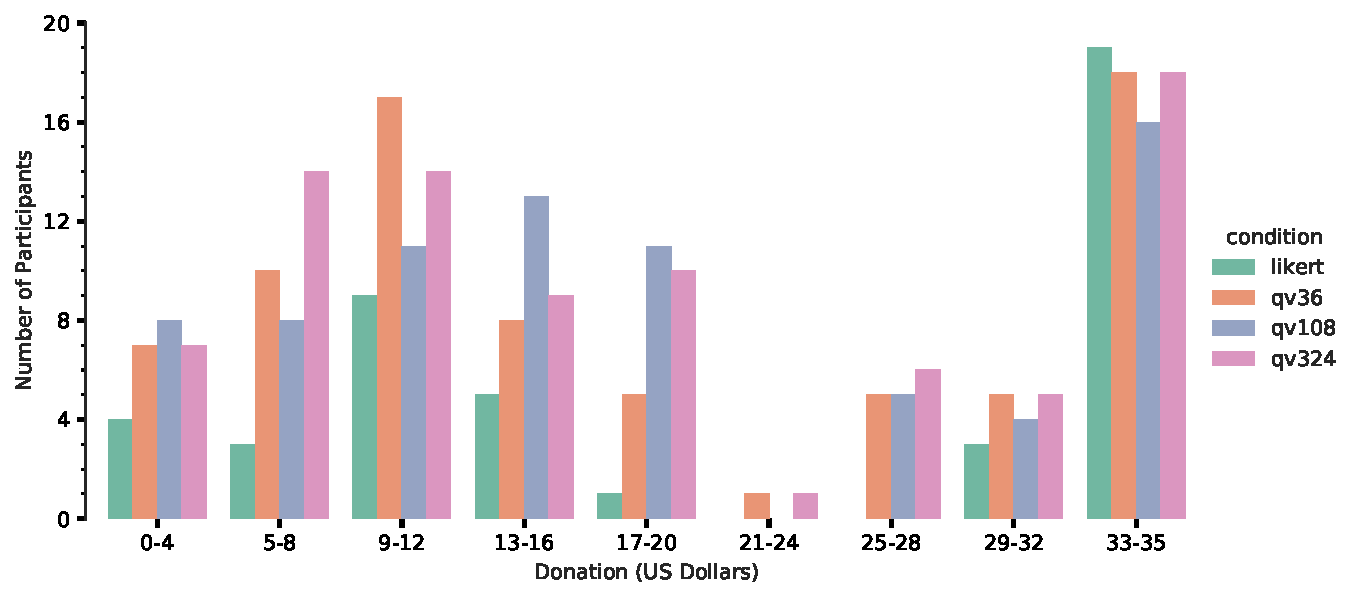
\includegraphics[width=\textwidth, keepaspectratio=true]{content/image/total_contributions_across_conditions.pdf}
    \caption{
       Distributions of Total Donation Amounts across Conditions
    }
    \Description[Distributions of Total Donation Amounts across Groups for experiment 1]{Distributions of Total Donation Amounts across Groups for experiment 1}
    \label{fig:total_don_exp1}
\end{figure}

Given the aggregated total donation amount across all the participants in each condition, the amount was distributed to the nine charities in a highly varying manner as shown in Figure \ref{fig:topic_don_exp1}. The environment-related, health-related, and human-related charities were consistently the most popular ones among all the options in different groups, while the art-related, international-related, and faith-related ones were always the least popular. However, we could see some differences in the population-level preferences towards charities across the four conditions. For example, the pets-related charity received far less donation in percentage than the three QV groups. This suggests that there was a good amount of variance in people's opinions towards the nine topics, making the surveying task meaningful.

\begin{figure}[htpb]
    \centering
    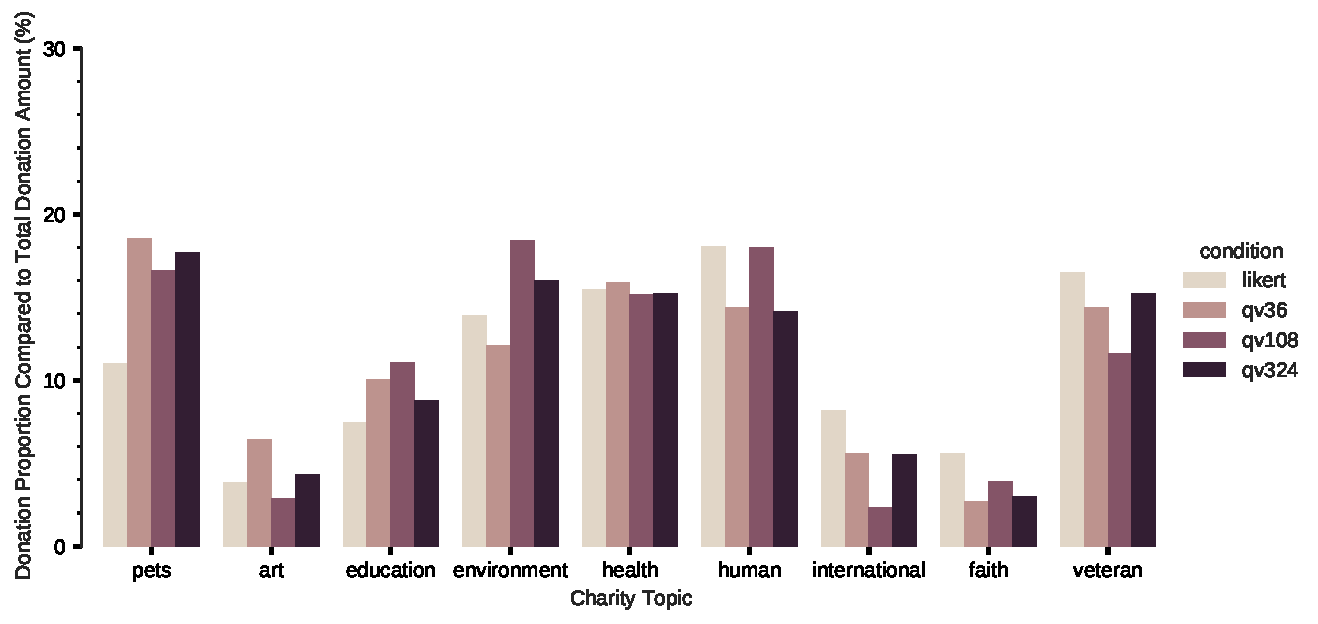
\includegraphics[width=\textwidth, keepaspectratio=true]{content/image/normalized_contributions_per_topic_across_conditions.pdf}
    \caption{
      Percentage Contribution Amount per Topic with Respect to the Total Donation Amount across Conditions
    }
    \Description[Percentage Contribution Amount per Topic with Respect to the Total Donation Amount across Conditions for experiment 1]{Percentage Contribution Amount per Topic with Respect to the Total Donation Amount across Conditions for experiment 1}
    \label{fig:topic_don_exp1}
\end{figure}

%     QV & Likert votes descriptive statistics: votes distribution per topic across groups, budget usage distribution across QV groups

Figure \ref{fig:likert_exp1} shows how Likert responses distribute at the aggregated level across the nine topics. With a 5-point Likert scale, we can see that most topics have a distribution that skews towards positive opinions, with a median of "Important" and "Very Important". Even though the medians of six out of nine topics are all "Important", the shapes of their distributions are different, suggesting different levels of support by the participants. The sufficient amount of variations shown across topics indicates that our prompt in the experiment that asked participants to be aware of the resource constraint and express their relative preferences worked as intended. 

\begin{figure}[htpb]
    \centering
    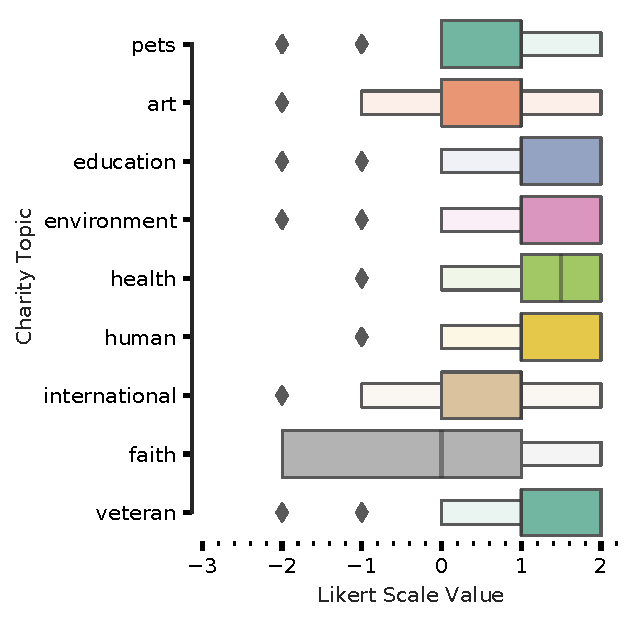
\includegraphics[width=0.4\textwidth, keepaspectratio=true]{content/image/likert_distribution_per_topic.pdf}
    \caption{
      Distribution of Likert Responses per Topic. Each level from -2 to 2 corresponds to Very unimportant, Unimportant, Neutral, Important, and Very important.
    }
    \Description[Distribution of Likert Responses per Topic for experiment 1]{Distribution of Likert Responses per Topic for experiment 1}
    \label{fig:likert_exp1}
\end{figure}

Comparing across the three QV surveys, the response distributions are similar but have subtle differences. Consistent with prior work in QV \cite{quarfoot2017quadratic}, most distributions of all the topics are close to a Normal distribution. Looking only at the median of a distribution, the result from QV36 has less variation than those from QV108 and QV324, and resembles that from the Likert survey more. The medians of QV108 and QV324, on the contrary, clearly show nuanced differences across topics. Distributions in QV324 have longer tails than those in QV108, suggesting that participants did make use of the increased credits to express more extreme opinions at higher costs. A further examination in the percentage voice credits budget usage in three QV conditions (Figure \ref{fig:qv_budget_exp1}), we found that there was no decrease in the median percentage usage as the budget size increased (all around 98\%), but the tail of lower percentage usage in QV324 was longer than in the other two cases. This finding suggests that the extra credits provided to the participants were put to good use in most cases, and that participants were still comfortable with completing a QV survey with a large budget up to the order of $N^2$ ($N$ is the number of options in a survey) and complicated calculations with our QV interface. % mention the implication of longer tail in QV324 in discussion section: need to be aware of using an overly large budget and resulting in a worse tail

\begin{figure}[htpb]
    \centering
    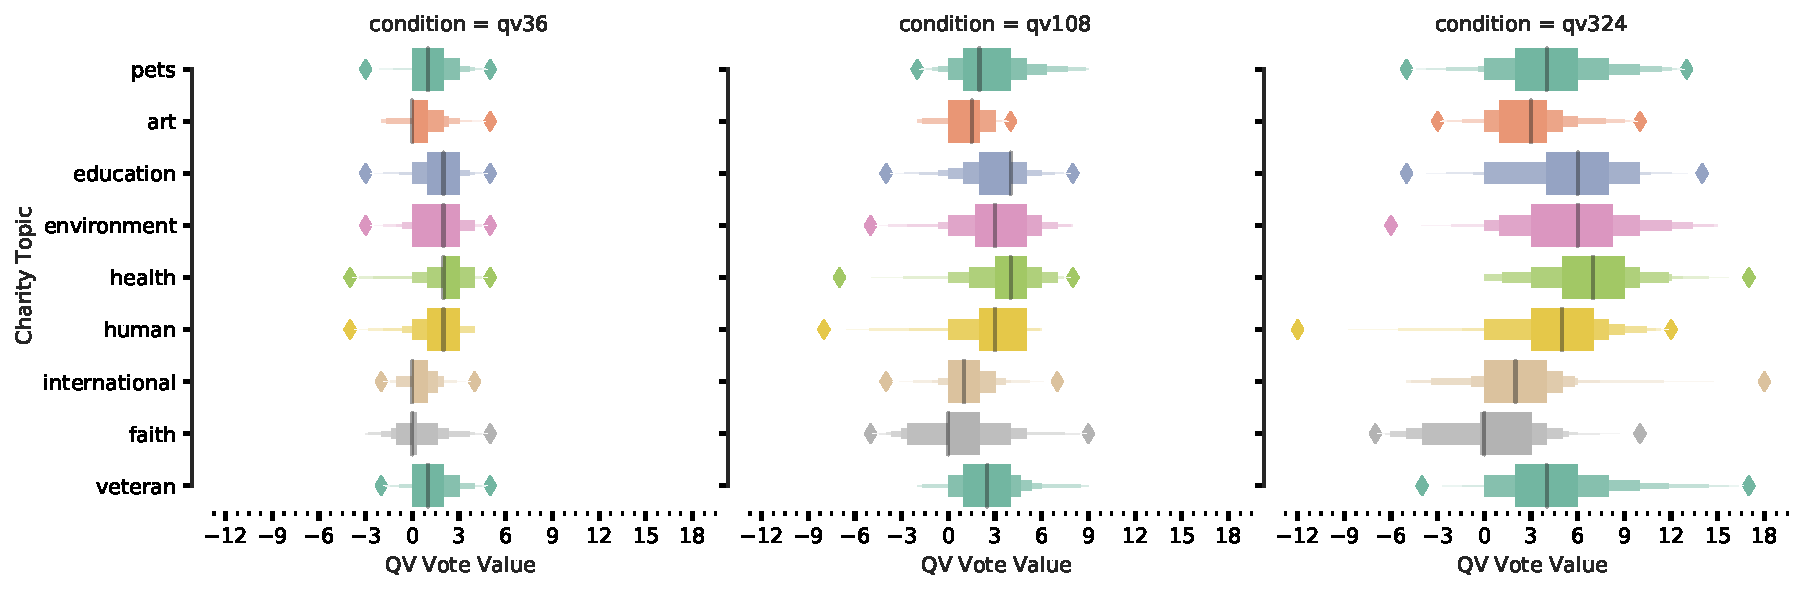
\includegraphics[width=\textwidth, keepaspectratio=true]{content/image/qv_distribution_per_topic.pdf}
    \caption{
      Distribution of QV Responses per Topic in QV36, QV108 and QV324. The maximum possible number of votes on a topic was 6 votes in QV36, 10 votes in QV108, and 18 votes in QV324.
    }
    \Description[Distribution of QV Responses per Topic for experiment 1]{Distribution of QV Responses per Topic for experiment 1}
    \label{fig:qv3_exp1}
\end{figure}


\subsubsection{Opinions Alignment Measurement Calculation}
% -- data transformation to alignment measurement
%     describe the calculation of cosine similarity angle theta
%     mention our test of checking if other factors impact total donation amount -> absolute vs. normalized donation amount
%     show histogram and other descriptive statistics of the angle data

To answer our research question of how align Likert and QV survey responses are with people's true opinions reflected by their incentive-compatible (to-do: is it accurate to use this term here?) behavior, we need to design a metric that can measure the degree of alignment between the two. Before discussing about our choice of metric, we need to clarify the definition of "alignment" used here. Our definition of having a perfect alignment between a set of survey response and a set of donation amount by the same individual is that the individual expresses preferences with the same relative strength in both cases. Formally, it is defined as the following:\par

\begin{quote}
    A set of survey response $\vec{v} = [v_1, v_2, ..., v_n]$, and a set of donation amount $\vec{d} = [d_1, d_2, ..., d_n]$, where $n$ is the number of topics or options involved in the decision, are perfectly align if there exists a positive constant $k>0$ that satisfies $k\vec{v} = \vec{d}$.
\end{quote}

Our alignment focused on the relative strength in opinion for two reasons. First, the results from our four sets of surveys and the donation task were not on the same scale. For example, the maximum possible number of votes on a topic in QV36 is 6 while the maximum donation amount on a topic is \$35. Second, given two participants with the same opinion across the nine topics, their total amount of donation may still differ due to other factors such as income level, level of education, etc. Even if both of them split their total donation amounts in the same way proportionally, their absolute donation amounts across the topics would be different. Hence, we decided to care only about the relative strength in opinions across topics.

The metric for measuring the degree of alignment thus need to be monotonic with respect to the amount of discrepancy between two preference vectors in terms of relative strength in preferences. It would be preferable if the metric is easily interpretable. With these two criteria in mind, we decided to use the angle $\theta$ in the Cosine similarity metric as the alignment metric. It is formally defined as the following: \par

\begin{quote}
    The Cosine similarity angle $\theta$ between a set of survey response $\vec{v} = [v_1, v_2, ..., v_n] \in \mathbb{R}^n$, and a set of donation amount $\vec{d} = [d_1, d_2, ..., d_n] \in \mathbb{R}^n$, where $n$ is the number of topics or options involved in the decision, is calculated via $\theta = \frac{180}{\pi} \arccos{\frac{\vec{v} \cdot \vec{d}}{\|\vec{v}\| \|\vec{d}\|}}$, and $0\deg \leq \theta \leq 180\deg$.
\end{quote}

Cosine similarity is a commonly used similarity metric that measures the cosine of the angle between two non-zero vectors \cite{singhal2001modern}. It only provides information about the relative orientation of the two vectors and does not take into account the magnitude of the vectors. The angle of the Cosine similarity measures the same thing but represents it in terms of the angle degree, instead of a value between 0 and 1, which makes it more intuitive for interpretation. The definition of the angle of Cosine similarity fits our need perfectly. It is monotonic with respect to how different the orientations of the two vectors are, i.e., the relative strength in opinions, and does not care about the magnitude of the vectors, i.e., absolute vote or donation amount. Two sets of perfectly align opinions will yield a Cosine similarity angle of zero, while two sets of completely opposite opinions will result in an angle of 180 degree.

To compare the degree of alignment between the survey results from Likert, QV36, QV108, QV324 and their corresponding truthful preferences reflected in the donation task, our first step was to compute a Cosine similarity angle for each participant in each group. For the Likert group, we computed the Cosine similarity angle of a vector of Likert responses (between -2 and 2 for each topic) and a vector of the absolute donation amount of the same individual. In the 3 QV conditions, the angle is between a vector of QV votes and a vector of the absolute donation amount of the same participant. The next step that completes our analysis is setting up a Bayesian Model for these four sets of Cosine similarity angle per condition as described in the next subsection.


\subsubsection{Bayesian Formulation}
% -- Bayesian formulation
%     why Bayesian
%     the type of analysis question
%     choice of the likelihood function
%     choice of prior distributions

Given the four sets of Cosine similarity angle under Likert, QV36, QV108 and QV324 conditions respectively, we employed a Bayesian formulation of the problem to compare the degree of alignment between pairs of the conditions. \textcite{kay2016researcher} introduced a few potential benefits for applying Bayesian analysis in the HCI community. A recent study by \textcite{xiao2019should} justified their use of Bayesian formulation with two additional reasons. Based on benefits proposed by past studies, we argued for our choice of Bayesian formulation with the following three reasons:

\begin{itemize}
    \item \textbf{Transparency and Fewer Assumptions} In a t-test or ANOVA, the data needs to follow several assumptions, including Normality and Homogeneity of variance. In our case, both assumptions may be violated. Hence, we used Bayesian formulation to relax the assumptions of normality and equal variances by defining a non-normal likelihood function and making variances independent across groups.
    \item \textbf{Small $n$ Studies} Traditional statistical tests that assume Normality require at least a sample size of 30. Even when a sample size is greater than 30, a large effect size may still produce an insignificant p-value due to a not sufficiently large sample. On the contrary, a Bayesian model is valid at every value of $n$. Given the relatively small sample of our Likert group, we chose to use a Bayesian model.
    \item \textbf{Additional Information} Compared to traditional statistical analysis that only produce a single p-value and a single effect size value, a Bayesian model is able to produce the entire distribution of the effect size, making additional information available for clearer inference. In our study, effect size is in particularly important because the cost of switching to a new survey tool is not worthwhile if the effect size is not substantial even if we get a significant p-value.
\end{itemize}

In our Bayesian formulation, the outcome variable $\theta_{i|j}$ is the Cosine similarity angle between a survey response vector and a donation amount vector of each participant $i$ under a given experimental condition $j$: Likert donation alignment, QV36 donation alignment, QV108 donation alignment, QV324  donation alignment. Our goal is to first find four best fitting distributions that describe the four sets of $\theta_{i|j}$ respectively, then compare the means of each pair of distributions to see if they differ significantly and substantially via Bayesian analysis. 

\begin{figure}[htpb]
    \centering
    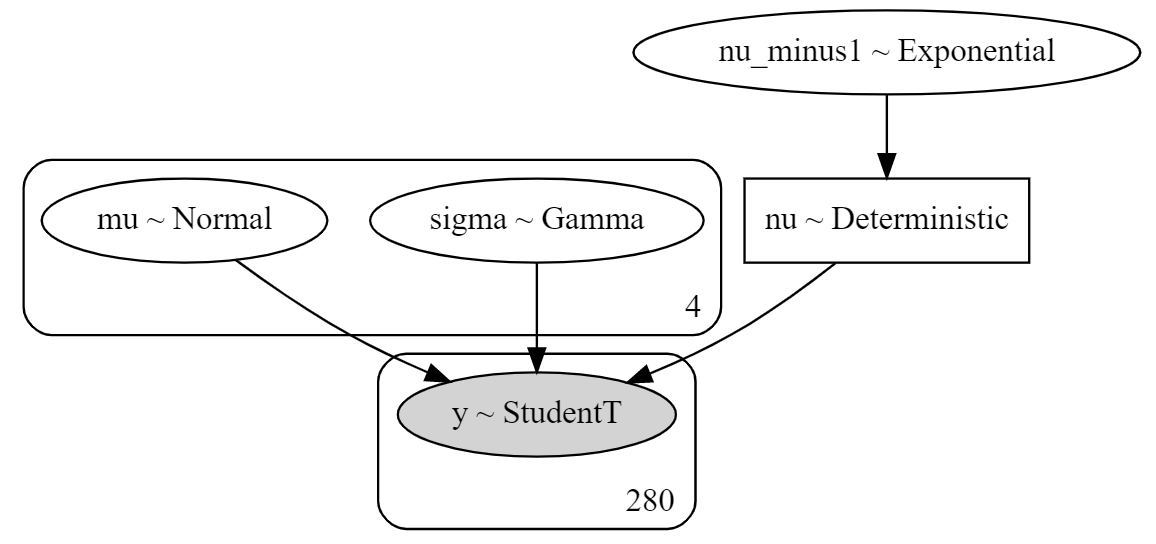
\includegraphics[width=0.8\textwidth, keepaspectratio=true]{content/image/model_graph.png}
    \caption{
      Graphical representation of our Bayesian model (to-do: update to a prettier version)
    }
    \Description[Graphical representation of our Bayesian model for experiment 1]{Graphical representation of our Bayesian model for experiment 1}
    \label{fig:bayesian_model_exp1}
\end{figure}

We chose a Student-t distribution to describe the Cosine similarity angle data per condition, i.e., as the likelihood function in the Bayesian model (note that this is a drawing distribution, not the t-test). A Student-t distribution is similar to a Normal distribution in the overall shape but is heavy-tailed, which is more forgiving about having more extreme values than a Normal distribution with the same variance. We did not want to make the strong assumption of Normality and thus decided on a Student-t distribution. In Bayesian modeling, typically, the likelihood function is parametric, meaning that each parameter of the likelihood function is treated as a random variable drawn from a distribution with parameters, i.e., what we also called the prior of the likelihood model parameters. In a Student-t distribution of a given condition $j$, there are three parameters: the mean ($\mu_j$), the scale ($\sigma_j$), and the degrees of freedom ($\nu$). In general, we defined the priors, i.e., likelihood functions of the parameters, based on the criterion of being weakly informative since we did not want to impose any strong assumption on what the model should look like and preferred allowing all possible values for the parameters. The detail Bayesian model is the following (also in Fig. \ref{fig:bayesian_model_exp1}:

\begin{quote}
    $\theta_{i|j} \sim$ Student-t$(\nu, \mu_j, \sigma_j)$, \hfill likelihood function to model angle in condition $j$ (1) \\
    $\nu \sim 1 + exp(\lambda)$, \hfill degrees of freedom (2) \\
    $\mu_j \sim N(M_0, SD_0)$, \hfill modal angle in condition $j$ (3) \\
    $\sigma_j \sim \Gamma(\alpha, \beta)$, \hfill scale parameter for condition j (4)
\end{quote}

We drew the degrees of freedom $\nu$ from a shifted exponential distribution to ensure that $\nu \geq 1$. The mode $\mu_j$ for condition $j$ was drawn from a Normal distribution with mean $M_0$ and scale $SD_0$, where $M_0$ and $SD_0$ were constants that were weakly informative. The scale parameter $\sigma_j$ was drawn from a Gamma distribution with generous $\alpha$ and $\beta$ constant values to ensure the scale parameter was always greater than zero. (to-do: do I need to specifiy what the constants are?) Now that we have finished introducing our Bayesian model, we will move on to the results of our analysis.

\subsubsection{Results Analysis}
    
% -- Results analysis
%     Tools: PyMC3, MCMC, NUTS
%     Describe fitted values & convergence (trace plots)
%     Describe effect size analysis for comparing Likert and QV
%     Describe effect size analysis for comparing across QVs

The Bayesian analysis was performed using PyMC3 \cite{salvatier2016probabilistic}, a popular Bayesian inference framework. One of the common computational techniques for Bayesian inference is Markov Chain Monte Carlo (MCMC), a stochastic sampling technique. It samples the posterior distribution $P(\theta | D)$, the distribution functions of the parameters in the likelihood function given the data observations $D$. We used the No-U Turn Sampler (NUTS) specifically in our analysis. 

\begin{figure}[htpb]
    \centering
    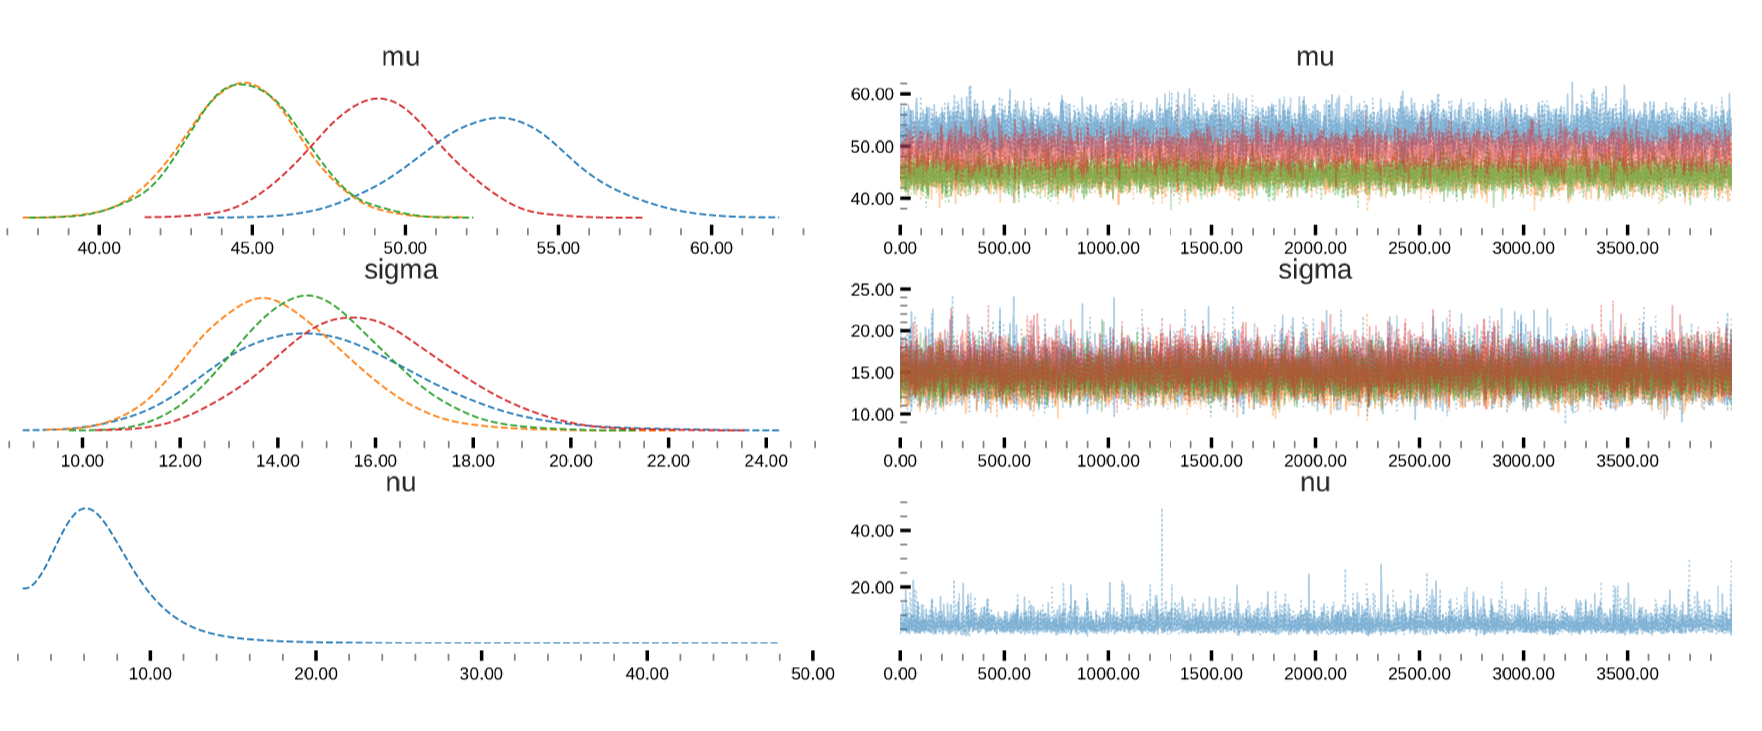
\includegraphics[width=\textwidth, keepaspectratio=true]{content/image/traceplot.png}
    \caption{
      Traceplot showing the results of the MCMC estimation. Left column is the posterior distributions for $\mu_{1-4}$, $\sigma_{1-4}$, and $\nu$, and right column shows the corresponding traces. (to-do: change to latex expression in figure; more explanation in caption)
    }
    \Description[Traceplot for experiment 1]{Traceplot for experiment 1}
    \label{fig:traceplot_exp1}
\end{figure}

Based on the traceplots in Fig. \ref{fig:traceplot_exp1}, the model shows good convergence. The Gelman-Rubin statistic $\hat{R}$ for all parameters were 1, indicating that the multiple sampling chains converged. Based on the posterior distributions in the left column in Fig. \ref{fig:traceplot_exp1}, we can see that the means of the four Student-t distributions vary. In the condition QV108 and QV324 (the orange and green lines), the modes of the mean of the Cosine similarity angle (QV108: $44.649 \deg$, QV324: $44.796 \deg$) are smaller than those in the other two conditions, indicating a better alignment between the survey results and donation behavior. QV36 (the red line) has a mode of the mean in the middle ($49.029 \deg$), and Likert (the blue line) has the largest mode of the mean ($52.857 \deg$) among all four conditions. The posterior distributions of the scale parameter in all four likelihood functions are similar, with a mode ranging from 13.904 and 15.724. (to-do: add posterior check in the appendix)

To further confirm how different the means of the likelihood functions between each pair of the conditions are, we constructed the distribution of the un-normalized difference and the distribution of the effect size (normalized difference) between the means. Figure \ref{fig:contrast_exp1}


\begin{landscape}[hbt]
    \centering
    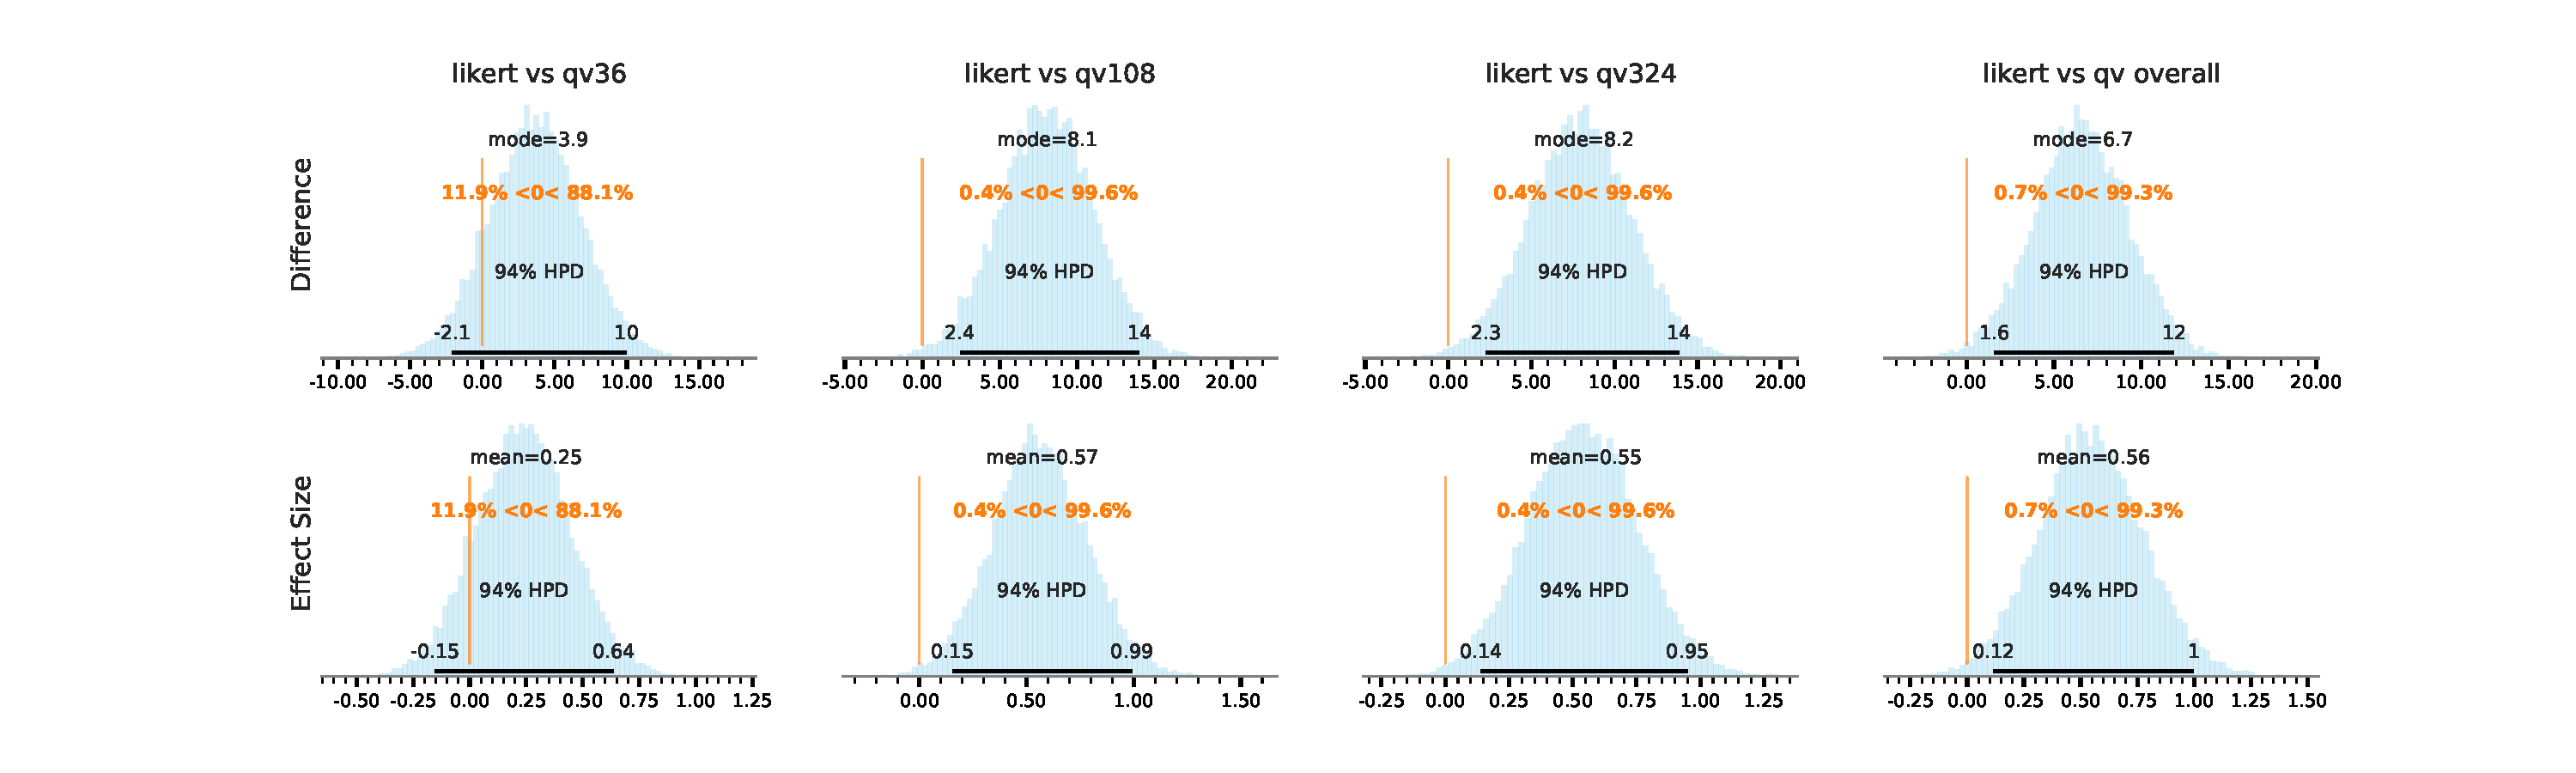
\includegraphics[width=1.4\textwidth, keepaspectratio=true]{content/image/Votes_vs_Absolute_Donation_StudentT_differences_and_effects.pdf}
    % there were issues with this caption, removed for now    
    % \caption{
    %   The figure shows comparison of the means from the survey-donation alignment likelihood function between the four experimental conditions (Likert donation alignment, QV36 donation alignment, QV108 donation alignment, QV324 donation alignment). The last column shows contrasts between the Likert donation alignment and the pooled QV donation alignment across three QV conditions. The first row focuses on the un-normalized difference while the second row is about the effect size. Since we are highlighting contrasts, each sub-figure shows an orange vertical line located at 0. 
    % }
    \Description[Contrasts for experiment 1]{Contrasts for experiment 1}
    \label{fig:contrast_exp1}
\end{landscape}
    
\subsection{Experiment 1 Qualitative Analysis Results}\label{results-1-qual}
We ask participants to provide a freeform text response on the reason why they made the choices they made
when participants filled out the Likert scale survey or QV survey,
Of all surveys ($N=394$) across both groups, most participants filled out the surveys ($N=331$) based on what they think are the most important issues to them. %84 percent
Besides, a small portion of participants ($N=30$) used their instincts when replying to the survey.
Some participants either think that every aspect is important ($N=7$) or that resources should be equally distributed ($N=7$).

